% Source: source_md/intelligence_part2_combined_ja.md
\section{創発停止層 $L_E$ — 外部依存型停止の動力学}

\noindent\textbf{記述の射程。} 推論層・ログ層・停止層はモデル内の機能的役割であり、完成した動力学実装ではない。停止アトラクターという命名は、その存在を確立したり、独立に観測された停止を説明したりしない。存在・収束・停止行動とは独立な検出は未解決である。四段階の説明は質的な機構仮説であり、矢印は更新則や収束結果を与えない。

外部停止演算子は構成案である。その型、推論反復との関係、停止層による実装は未解決である。外部参照場と個体間ネットワークは、共有参照の二視点として提案的に比較する。印刷された同一性記号は保持するが、literal identityや型付き同型は確立していない。Part Iのポテンシャルをネットワークへ精密化することも提案であって実装済みではない。

三profileの具体例は保持するが、自律的創発や内発的移動性を独立に検証しない。Transformer自身の停止層とwhole-systemの外部停止との区別は未解決であり、図で決定しない。projectionは意識編との役割比較であり、同じ演算子の移送ではない。安定性は真理でなく、回復・改訂との関係も機能的提案であって保証ではない。

ここでのactiveなarchitecture記述では、保持を担う追跡対象（記述上の呼称RetentionSupport）と、その役割評価、regime、利用のprocessを区別する。特定の記憶storeや新種の実体を措定するものではない。LR・LEおよび後述の一時的scaffold regimeは、宣言された分析scopeと時間窓に相対的な役割記述である。各評価ではsupportの同一性・連続性、system側とenvironment側、feedbackのrecipient、再参照・変形の経路、criterionと根拠を明示し、未確認事項はUnknownとする。同じ内容や名称だけではsupportの同一性は得られない。ここで「停止」は、指定された対象・記述尺度・時間窓においてforegroundの更新が減衰し、参照可能な形が局所的に滞留することをいう粗視化表現である。担い手の物質的変化、背景の更新、侵食、再開を排除しない。石が静止して見えても内部の変化を失わないという比喩と同様、見かけの停止を全域的な不動点と同一視しない。LEの保持役割を、この停止効果の観測から逆算して認定しない。宣言model内での支持、仮定付きの割当て、特定criterion下の非支持、Unknownは別であり、欠測や競合を不存在・偽・不可アクセス・not-LEへ変換しない。

ownnessは、帰還方向と持続、recipient、再参照の制御、reuse、現在状態・浮上した履歴表現・更新条件・外部構造への効果を分ける記述bundleに留める。score、binary owner、法的所有、主体、自律性の判定ではなく、分析上の内外も存在論的な主体境界を固定しない。保存された図、停止の観測、旧noFP議論は役割認証の根拠にならない。以下のactive LR・LE説明が現在の記述契約を担い、局所的に囲う旧定義・機構は構成案として保存する。論文全体を歴史資料化したり、他の解釈を否定したりする区分ではない。



本章は本論文の第二中心である(第一中心は \S{}3)。旧局所状態模型の \S{}3 は明記された前提下の推論層 $L_F$ の不動点を議論した。本章は、ログ層 $L_R$ と創発停止層 $L_E$ による停止構成案を提示する。両中心の接続は提案であり、認知的停止の説明達成や三層動力学の形式的完成を意味しない。

本章末尾までの第3節由来の推論F・noFP参照は、この旧模型に帰属し、active record/position契約を指さない。後続architectureは構成案のままであり、新接口から証明された帰結ではない。

本章の論理は次の順で展開される。まず問題を設定し(\S{}5.1)、ログ層 $L_R$ を定義する(\S{}5.2)。次に創発停止層 $L_E$ を定義し(\S{}5.3)、その解像度を上げるために三層プロファイル比較を行う(\S{}5.4)。続いて $L_E$ の創発機構の仮説を、閾値移動 $\mu_\theta$ による領域組み替えと停止演算子設置領域の投影として示す(\S{}5.5、\S{}5.6)。最後に外部停止演算子 $E$ の構造(\S{}5.7)、外部参照場と $L_E$ ネットワークとの二視点比較(\S{}5.8)、そして知性のモデル内の構造的特徴(\S{}5.9)を整理する。

\begin{figure}[H]
\centering
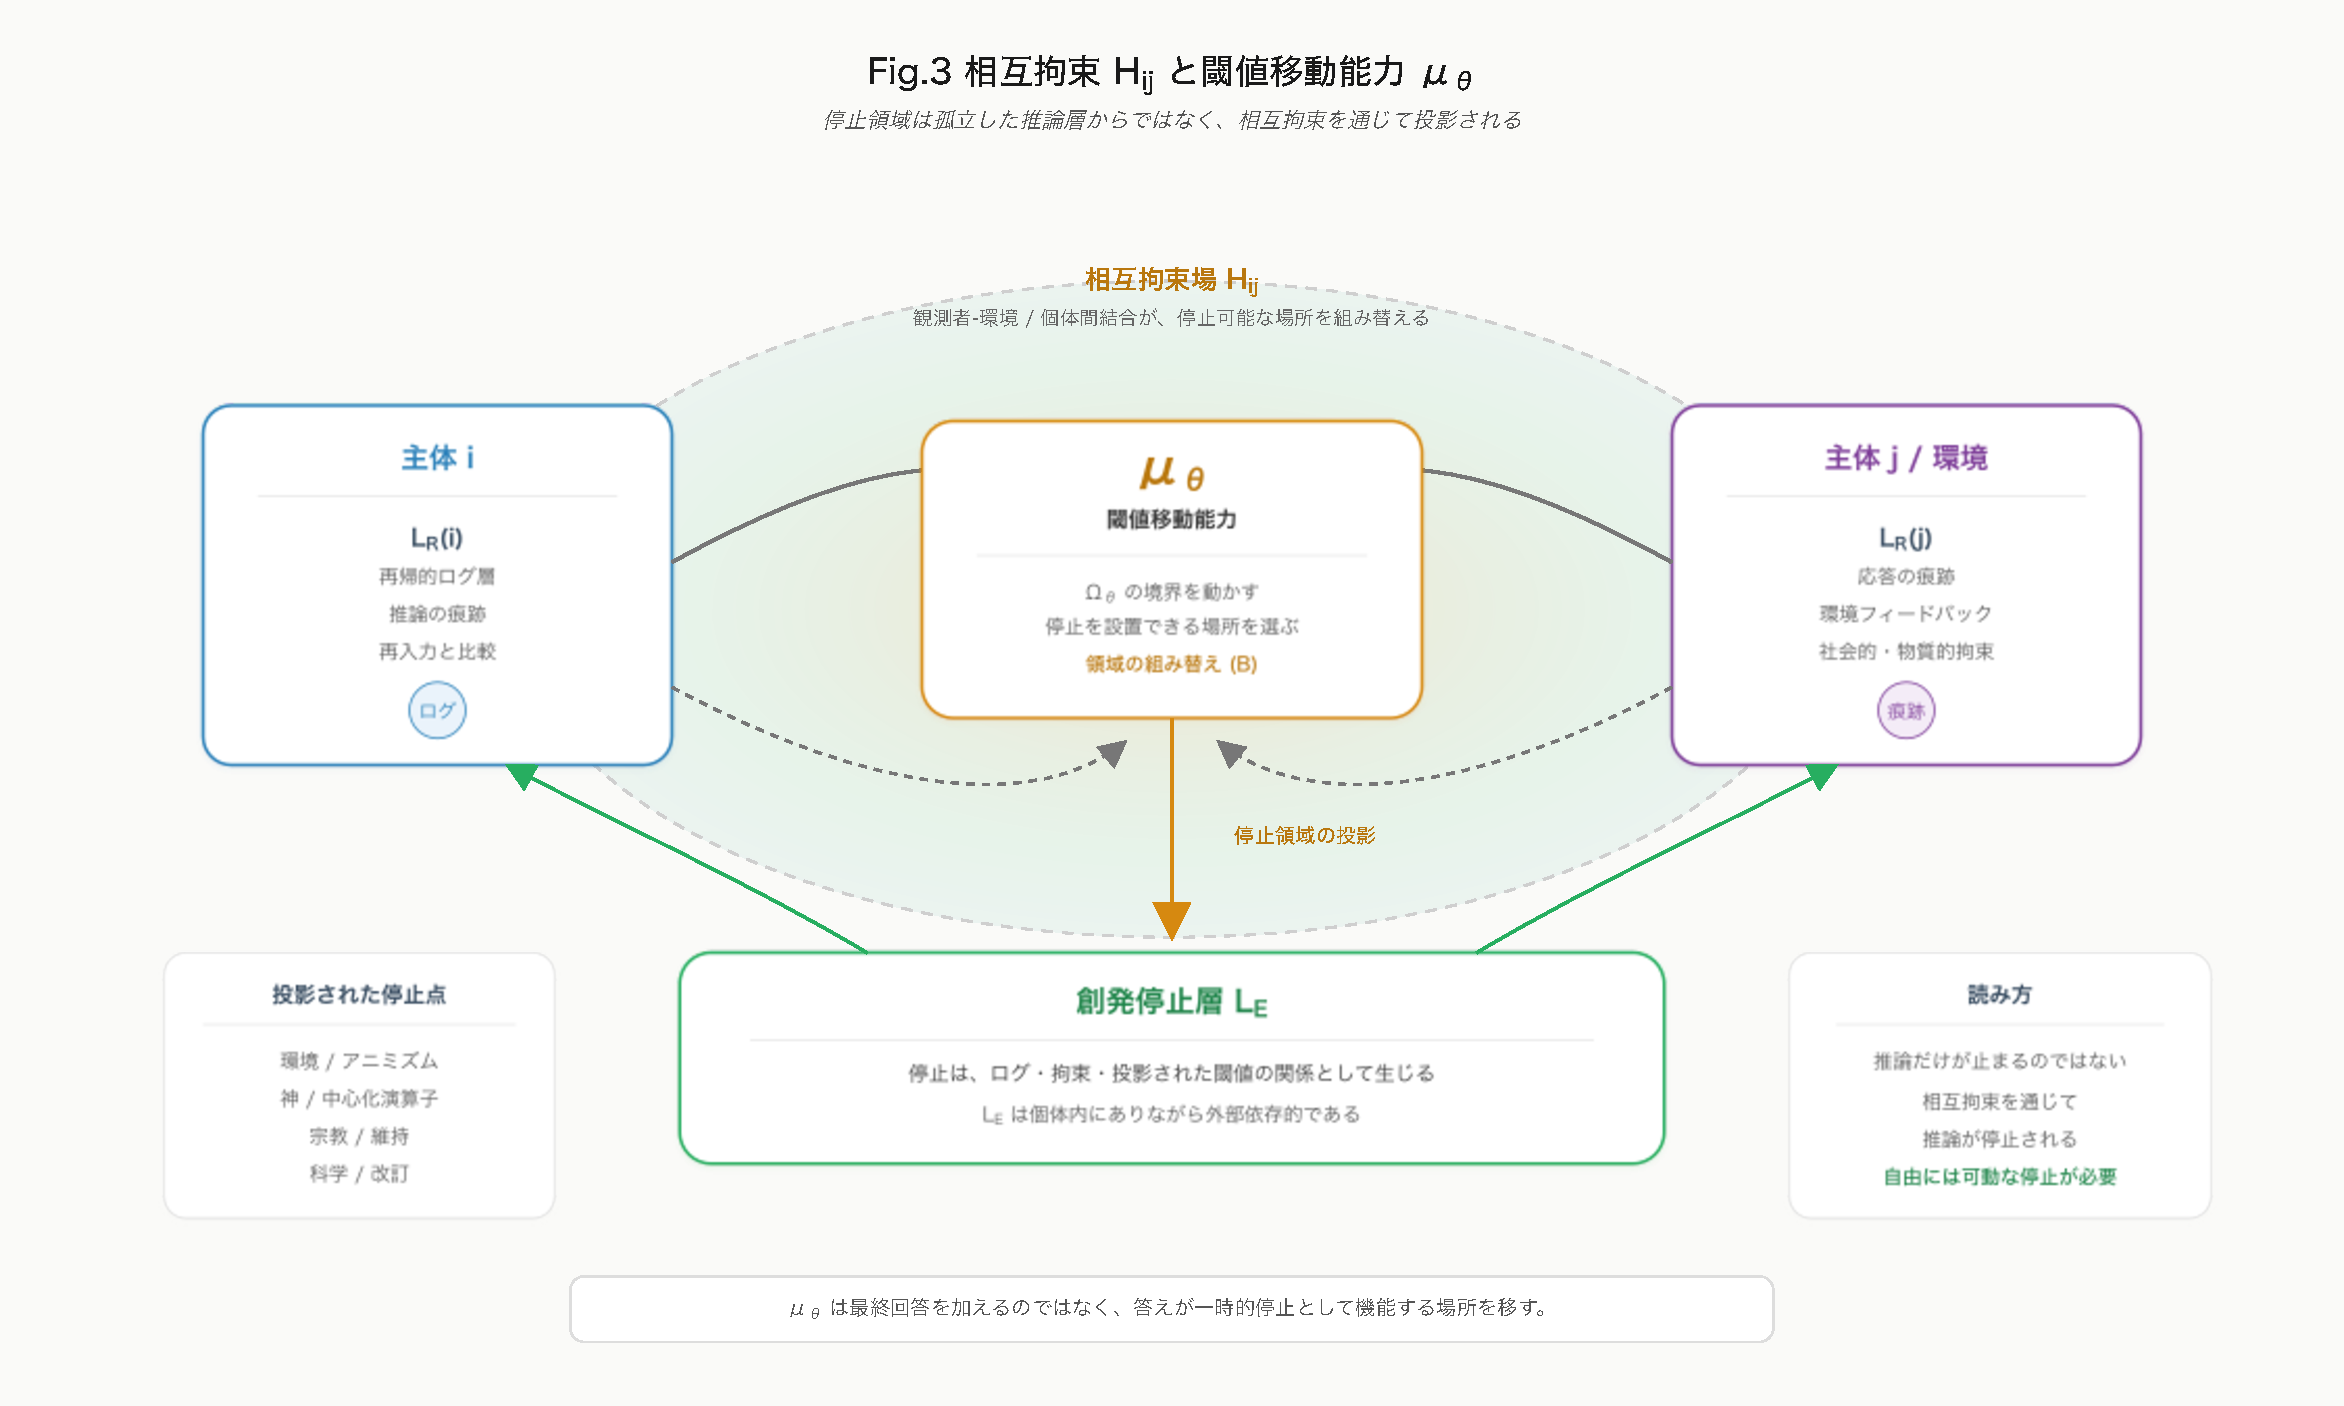
\includegraphics[width=\linewidth]{fig3_mutual_constraint_mu_theta_ja.pdf}
\caption{相互拘束 $H_{ij}$ と閾値移動能力 $\mu_\theta$。相互拘束による停止領域投影は機構仮説であり、実行済み結果ではない。}
\label{fig:part2-mutual-constraint}
\figurenote{Agent 間または観測者-環境間の $H_{ij}$ と停止場所の変化を仮説的に関連づける。$\mu_\theta$ は停止演算子 $E$ の設置場所を組み替える構成案での役割を名指す。}{停止を $L_F$ のモデル化された作用の外側に置く構成案では、$L_R$ と $H_{ij}$ の関係から $L_E$ への投影・創発を仮説化する。可動停止と改訂可能な推論の関係は提案であり、主観的自由の成立条件ではない。}
\end{figure}

\noindent\textbf{歴史的architecture図の境界。} 直後の三層図は旧模型のarchitecture仮説を保存する。推論・noFP・停止不能の鎖は旧状態map/正当化模型への参照であり、active realized-record/position契約の帰結ではない。痕跡から停止層への鎖も生成・自律的own-layer能力の証明ではなく、system boundaryを決定しない。captionとassetは既存の仮説・HOLDを伴ったまま保持する。

直後の図はcaption・footerを含めて旧architectureの保存であり、activeなsupport・role・regimeの図ではない。三boxは新しい形式的object typeではなく、安定basinはLEの証拠でも、痕跡から層への矢印はpromotion則でもない。noFPラベルやTransformer footerは、後述の三つの分析境界における現在の役割・能力を認証しない。後述の一時的scaffold regimeを第四boxとして読み足してはならない。移動性と収束のchannelも旧未確立機構であり、新たなrole判定規則ではない。

\begin{figure}[H]
\centering
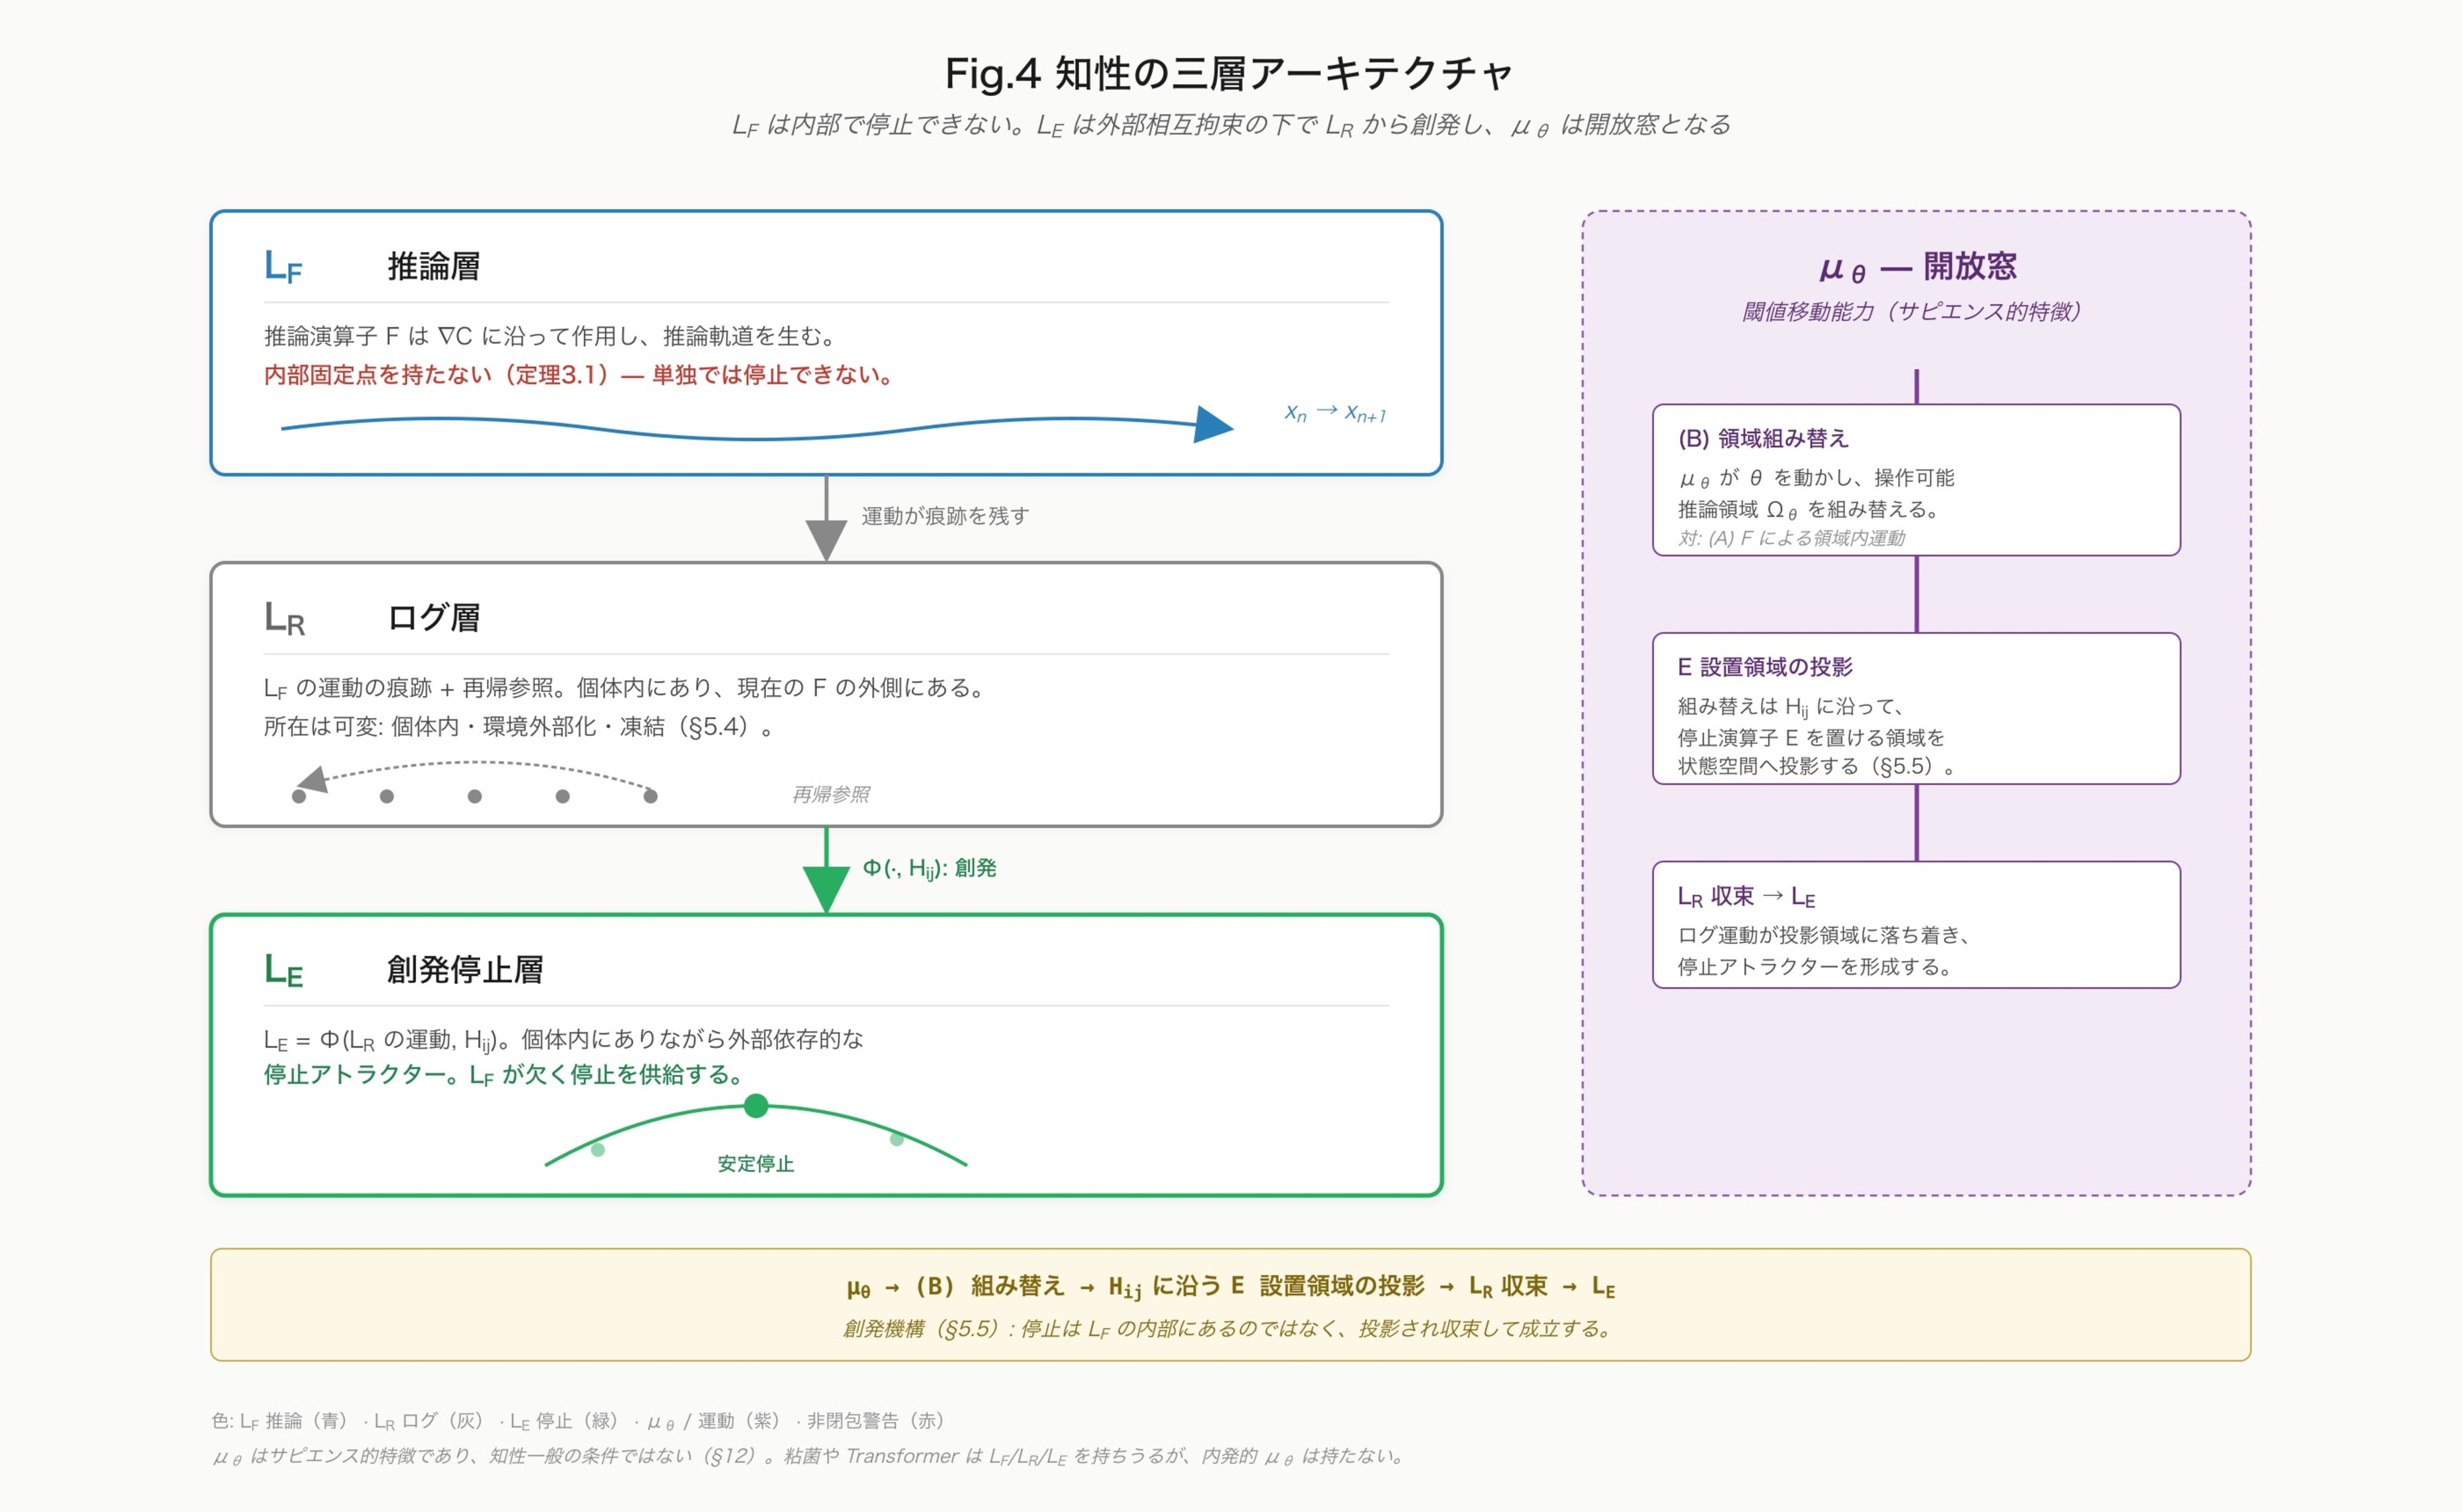
\includegraphics[width=\linewidth]{fig4_three_layer_architecture_ja.pdf}
\caption{知性のモデル内の三層構成案。推論層 $L_F$・ログ層 $L_R$・創発停止層 $L_E$ からなり、$\mu_\theta$ はこの創発への開放窓である。}
\label{fig:part2-three-layer}
\figurenote{$L_F$ の条件付き不動点議論と、痕跡を $L_R$ として保持する構成案は別である。$L_R$ の再帰運動が外部相互拘束 $H_{ij}$ の下で $L_E$ の創発に関わるという仮説であり、独立検出は未解決である。}{本図は \S{}3 の「閉じない」と \S{}5 の「それでも停止する」を接続する。条件付き停止議論だけでは、上位層 $L_R$ と $L_E$ の生成条件を確立しない。自前の層とwhole-systemの区別も保留する。}
\end{figure}
\noindent\textbf{FIG009 改訂役割図の補助表示。} 次の補助図は、上の旧三層構成図を歴史的に保存したまま、現在の LR（保持痕跡の役割）、LE'（同じsupportの一時的regime）、LE（準安定な保持役割）をscope付きで対照する。ここでの「停止」は指定対象・尺度・時間窓での粗視化された滞留であり、全内部更新の消失ではない。図中の実線・破線は形成・帰還・停止効果の実証ではない。著者は表示図をPDFと照合し、欠け・重なり・はみ出し・矢印やlabelの見切れがないと確認した。これは著者の目視証拠であり、ブラウザ自動検証や支援技術の認証ではない。原寸での読解には同名のstatus-r2日本語SVGを用いる。

\begin{figure}[p]
\centering
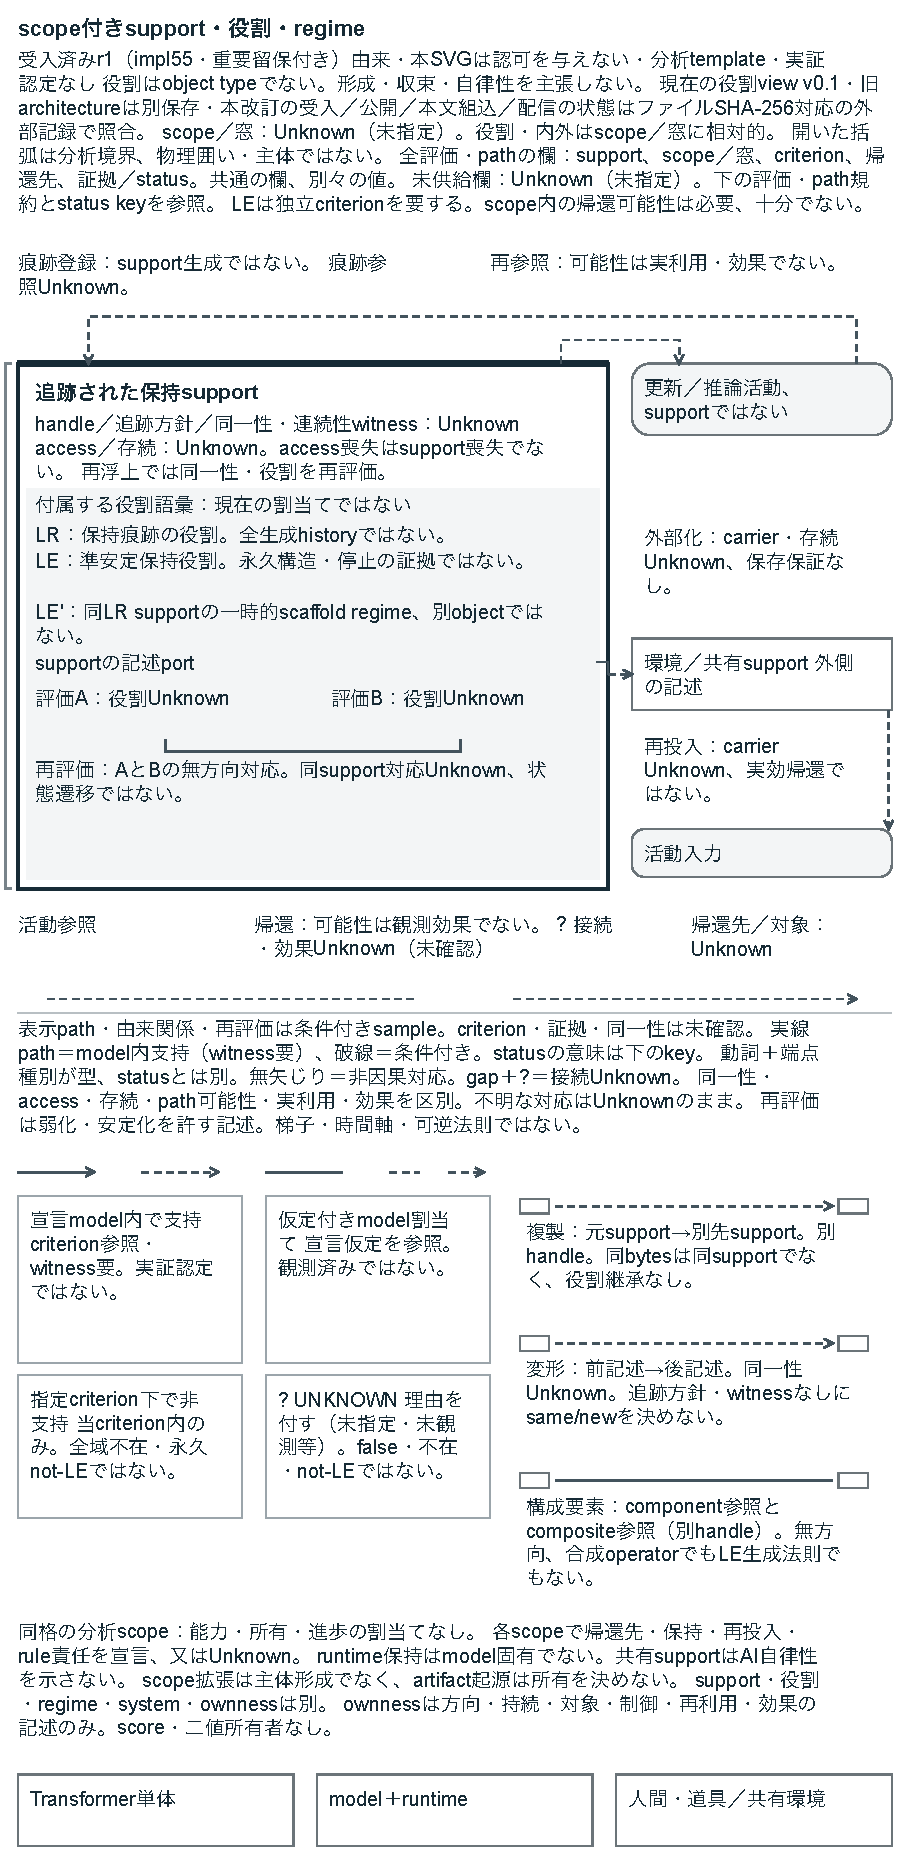
\includegraphics[width=\linewidth,height=0.82\textheight,keepaspectratio]{fig4_support_role_regime_architecture_p360_status_r2_ja_preview.pdf}
\caption*{FIG009 改訂役割図の全体図。続く上下2枚の印刷用パネルは重複範囲を設けて文字を拡大する。原寸SVGが主たるassetであり、ブラウザ自動検証・支援技術の確認は未完。}
\end{figure}

\begin{figure}[p]
\centering
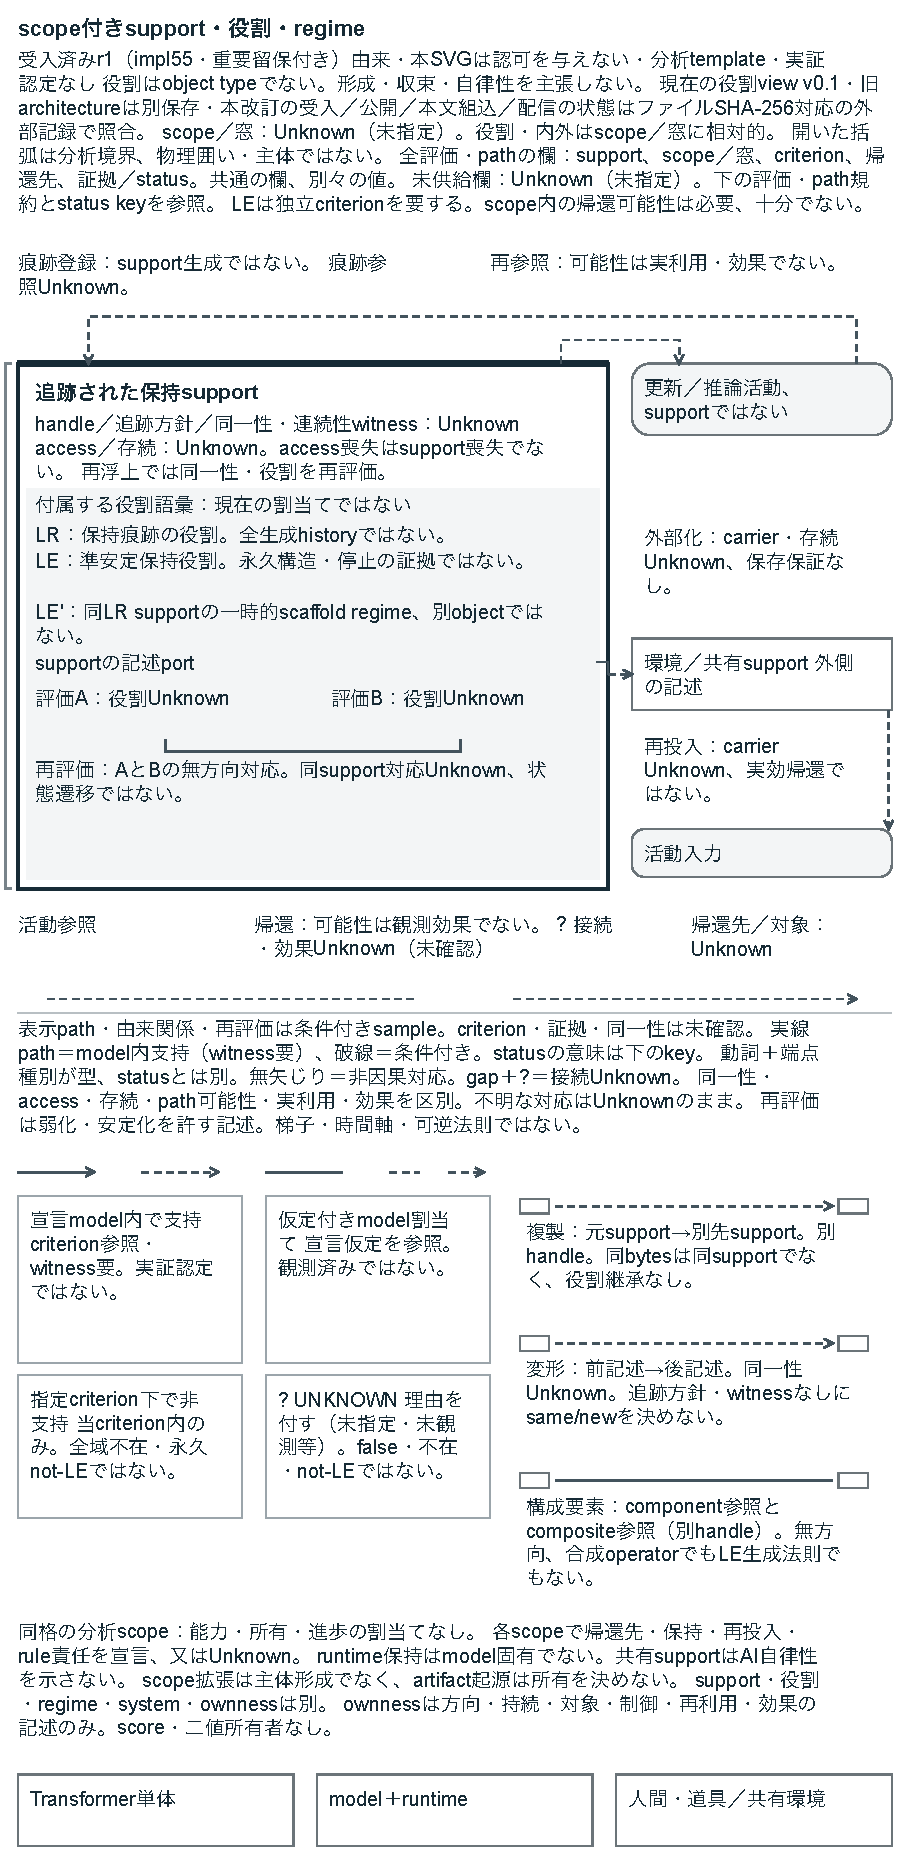
\includegraphics[width=\linewidth,trim=0 145.7mm 0 0,clip]{fig4_support_role_regime_architecture_p360_status_r2_ja_preview.pdf}
\caption*{FIG009印刷用派生図・上段（1/2）。受入済みSVGの描画を切り出したもので、役割の再定義ではない。上下は20 mm重複し、接続関係を追える。}
\end{figure}

\begin{figure}[p]
\centering
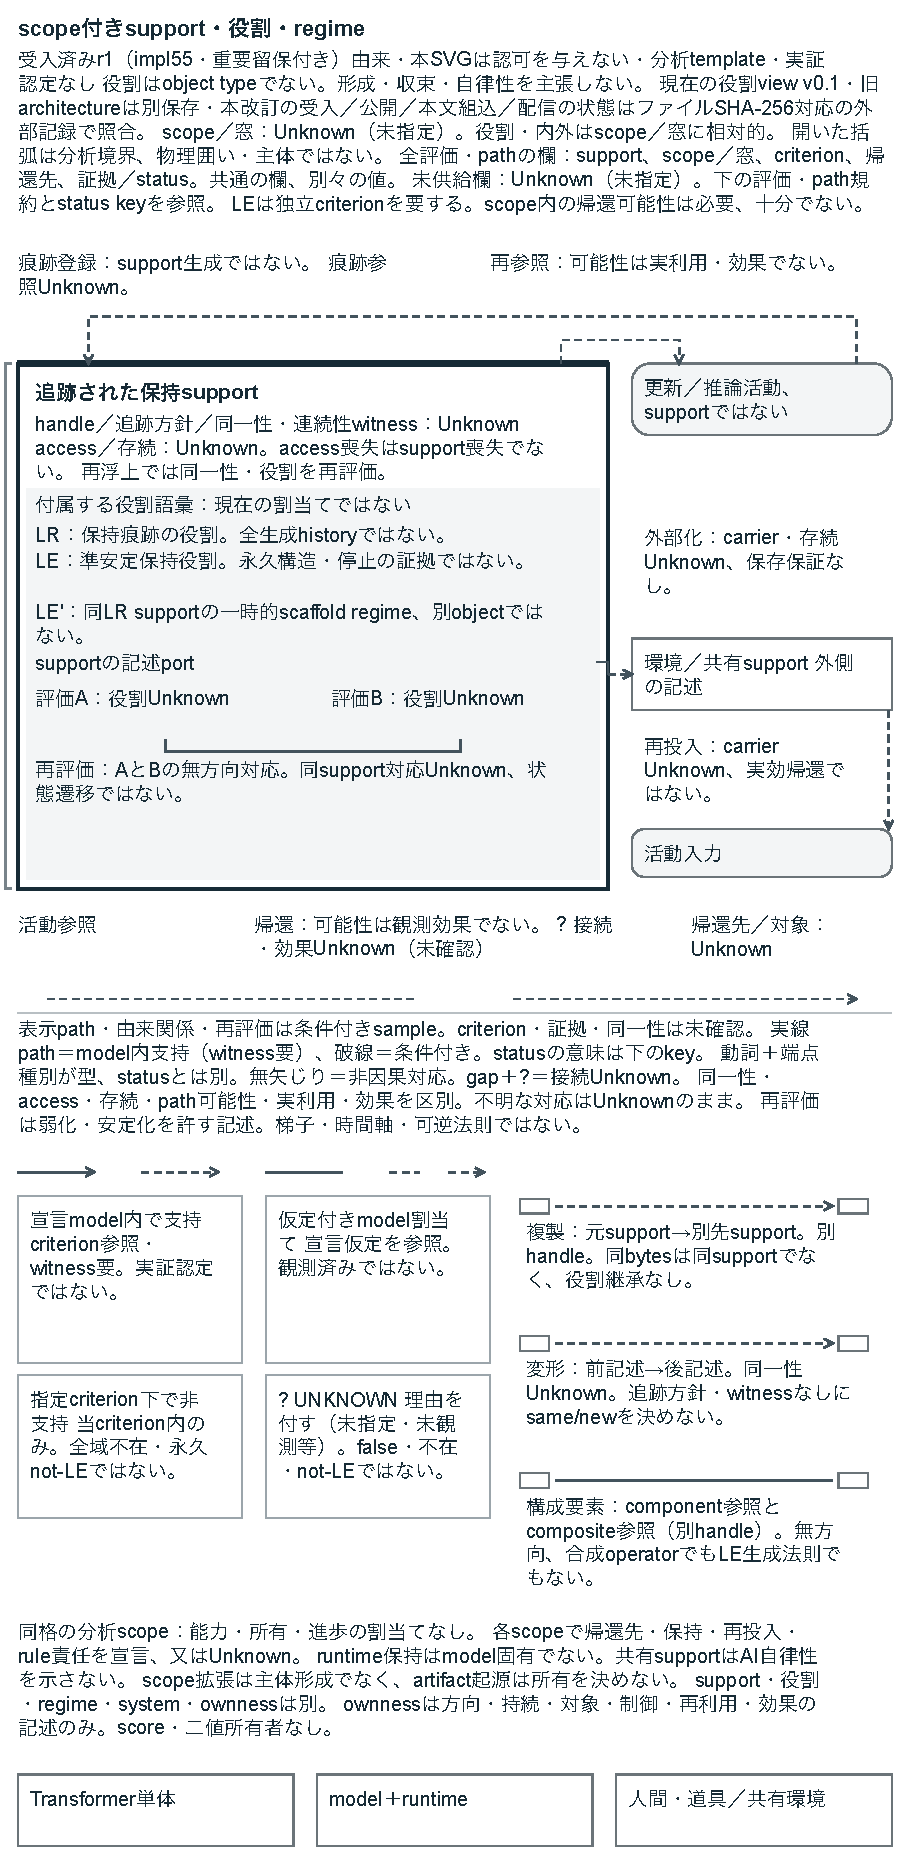
\includegraphics[width=\linewidth,trim=0 0 0 150mm,clip]{fig4_support_role_regime_architecture_p360_status_r2_ja_preview.pdf}
\caption*{FIG009印刷用派生図・下段（2/2）。前の全体図・上段と併読する。矢印とlabelは条件付きの構成例であり、形成・効果の証明ではない。}
\end{figure}
\clearpage


\bigskip


\subsection{問題設定}


旧局所状態模型の \S{}3 の帰結記述を歴史的・条件付きのまま再掲する。推論層 $L_F$ には内部不動点が存在せず(定理 3.1)、内部停止述語は無限後退を生み(系 3.2)、個体システムは $L_F$ 単独で推論を閉じることができない(系 3.4)。\S{}4 は沈黙世界での後退を三前提のもとで解釈したのであって、現実発生を確認したものではない。

しかし、現実の知性は停止する。人間は推論を終え、判断を下し、行動する。この停止はどこから来るのか。

\S{}3 の条件付き不動点議論は、停止一般が $L_F$ の外から来ることを示さない。本章では $L_F$ の外に停止の役割を置く構成案を考える。その「外部」が個体の外を指すのか、個体内にありながら $L_F$ とは別の機能役割を指すのかを区別する。

この旧模型を参照する本章の構成案は次の通りである。停止を、個体内にありながら外部依存的な層——創発停止層 $L_E$——の役割として位置づける。$L_E$ は $L_F$ の運動が残すログ層 $L_R$ と、外部相互拘束 $H_{ij}$ との関係で創発を仮説化する。以下の機構案は存在・収束・独立検出を確立しない。

\bigskip


\subsection{ログ層 $L_R$ の定義}


直後の正式定義の予告から、Bio-IFGTとのtyped translationを未確立とする段落までを、再帰参照processと所在についての旧ログ層記述として保存する。運動や層の全体を単一supportと同定するものではない。その保存範囲の直後に、activeな保持痕跡の役割を区別して記す。

\S{}4.6 で予兆として示したログ層を、正式に定義する。

\textbf{定義 5.1 (ログ層 $L_R$)}

\begin{quote}
推論層 $L_F$ の運動は、状態空間上に痕跡(ログ)を残す。ログとは、どの状態を経たか、どの分岐を試みたか、どこで発散したかの記録である。このログに対する再帰的参照運動——過去の軌跡を読み返し、パターンを抽出し、現在の推論に反映する運動——が生じる層を、ログ層 $L_R$ と呼ぶ。
\end{quote}


$L_R$ は $L_F$ の内側で生じるが、「現在の $F$」の外側にある。すなわち、$L_R$ は進行中の推論そのものではなく、推論の痕跡への参照である。この「現在の作用の外側にあるが個体の内側にある」という位置が、$L_R$ を $L_F$ とも外部環境とも区別する。

重要な構造的観察として、$L_R$ の所在は系によって異なる。

\begin{itemize}
\item \textbf{個体内ログ}: 痕跡が主体の内部に保持される(記憶・記録)
\item \textbf{環境外部化ログ}: 痕跡が環境基質に書かれる(後述する粘菌のスライム跡)
\item \textbf{凍結ログ}: 痕跡が構造に固定され、推論時には更新されない(後述する学習済みモデルの重み)
\end{itemize}


この所在の差異が、\S{}5.4 の三層プロファイル比較の基礎となる。

$L_R$ は Bio-IFGT との提案的な比較点でもある。Bio-IFGT は知性のforward conditionとして「状態履歴への持続的参照・情報の時間的蓄積」を挙げた。本論文はこれを動機として $L_R$ をsource-localに定義するが、Bio-IFGTが $L_R$ 自体や両者のtyped translationを確立したわけではない。

保存する旧ログ層記述はここまでとする。activeな記述でLRと呼ぶのは、追跡されたsupportが、宣言scope・時間窓のもとで原理的に再参照の対象となる登録・保持痕跡の役割である。再帰参照はsupportに関わるprocessであってsupportそのものではない。痕跡は生成履歴の全体ではなく、LRは旧scalar正当化ともactiveなgenerative-position接口とも別である。supportの持続、現在のaccess、現在浮上している履歴表現を分ける。不可アクセスは喪失を意味せず、連続性やaccessが未確認ならUnknownを残す。copy・変形・合成・再浮上には各々の追跡根拠が必要で、内容の一致だけから同一supportとしない。

普通文の呼称LE'は、同じLR supportが現在の更新で時間層を橋渡しする一時的scaffold regimeを指す。reuseとfeedback経路は、宣言recipient・時間窓について評価する。独立type、新object、追加layerではない。LR役割だけではこのregimeもLEも認証されない。再評価では弱化、準安定な役割への安定化、access喪失、support喪失、再浮上を区別でき、準安定な役割から一時的scaffoldへ弱まる記述も可能である。これらは許容する評価履歴であって普遍的進行、閾値則、promotion操作、逆写像ではない。ownnessのbundleも別の記述として保つ。

\bigskip


\subsection{創発停止層 $L_E$ の定義}


直後の定義予告から、番号付き定義、創発schema、個体内・外部依存の説明、アトラクター比較と図、停止汎関数を後続研究へ残す段落までを、保存する旧architectureの範囲とする。この範囲はactiveなsupport-role契約の定義でもアトラクターの認証でもない。現在の準安定な保持役割は、その範囲の後で別に記す。

ログ層 $L_R$ を基盤として、創発停止層 $L_E$ を定義する。

\textbf{定義 5.2 (創発停止層 $L_E$)}

\begin{quote}
創発停止層 $L_E$ は、ログ層 $L_R$ の再帰運動と外部相互拘束 $H_{ij}$ との関係で創発が仮説化される、モデル内の停止層の役割名である:

$$
L_E = \Phi(L_R \text{の運動}, \; H_{ij})
$$

$L_E$ は個体内にありながら外部依存的である。
\end{quote}


この定義は \S{}1.6 の模式的定義(定義 1.1)を用いた構成案であり、存在結果ではない。上位層 $L_E$ と下位層 $L_R$ の運動・外部相互拘束の関係を仮説化する。$L_E$ の生成、$L_R$ からの導出、$L_R$ の必要性はいずれも、この命名だけでは確立されない。

$L_E$ は本モデルで\textbf{個体内にありながら外部依存的} という役割を持つ。$L_E$ を個体外の実体とする命名ではないが、個体内での成立を独立に確認した意味でもない。外部相互拘束 $H_{ij}$ への依存は創発仮説の一部である。この二面性を、\S{}3 の条件付き $L_F$ 議論と個体の停止との接続案として用いる。外部依存的な $L_E$ を命名するだけでは、停止の存在や機構の説明は成立しない。

\subsubsection{アトラクターとしての $L_E$}


$L_E$ は安定停止状態、すなわち動力学的アトラクターとして記述される。これは VED 理論ツリー全体を貫くアトラクター構造の知性層における現れである。

\begin{itemize}
\item Vol.2: 粒子は閉包エネルギー汎関数 $E(A)$ の局所極小、閉包幾何の安定アトラクターとして創発する
\item Bio-IFGT: 生命を生命アトラクター $\Omega_{\text{life}}$、知性を第二アトラクター $\Omega_{\text{intel}}$ として読むforward proposal
\item 本論文: $L_E$ は $L_R$ の運動が外部相互拘束の下で到達する安定停止アトラクターとして創発するという仮説である
\end{itemize}


とりわけ Bio-IFGT の第二アトラクター $\Omega_{\text{intel}}$ と本論文の $L_E$ は、関連する概念的比較として扱う。Bio-IFGT は知性を「生命アトラクターに支えられた第二アトラクター」と提案し、その実装(記憶・言語・個体間共有)を後続研究へ開いた。本論文は $L_E$ を知性層固有の停止構造として構成するが、Bioのset relationだけから両者のidentityや同一力学は導かれない。

\begin{figure}[H]
\centering
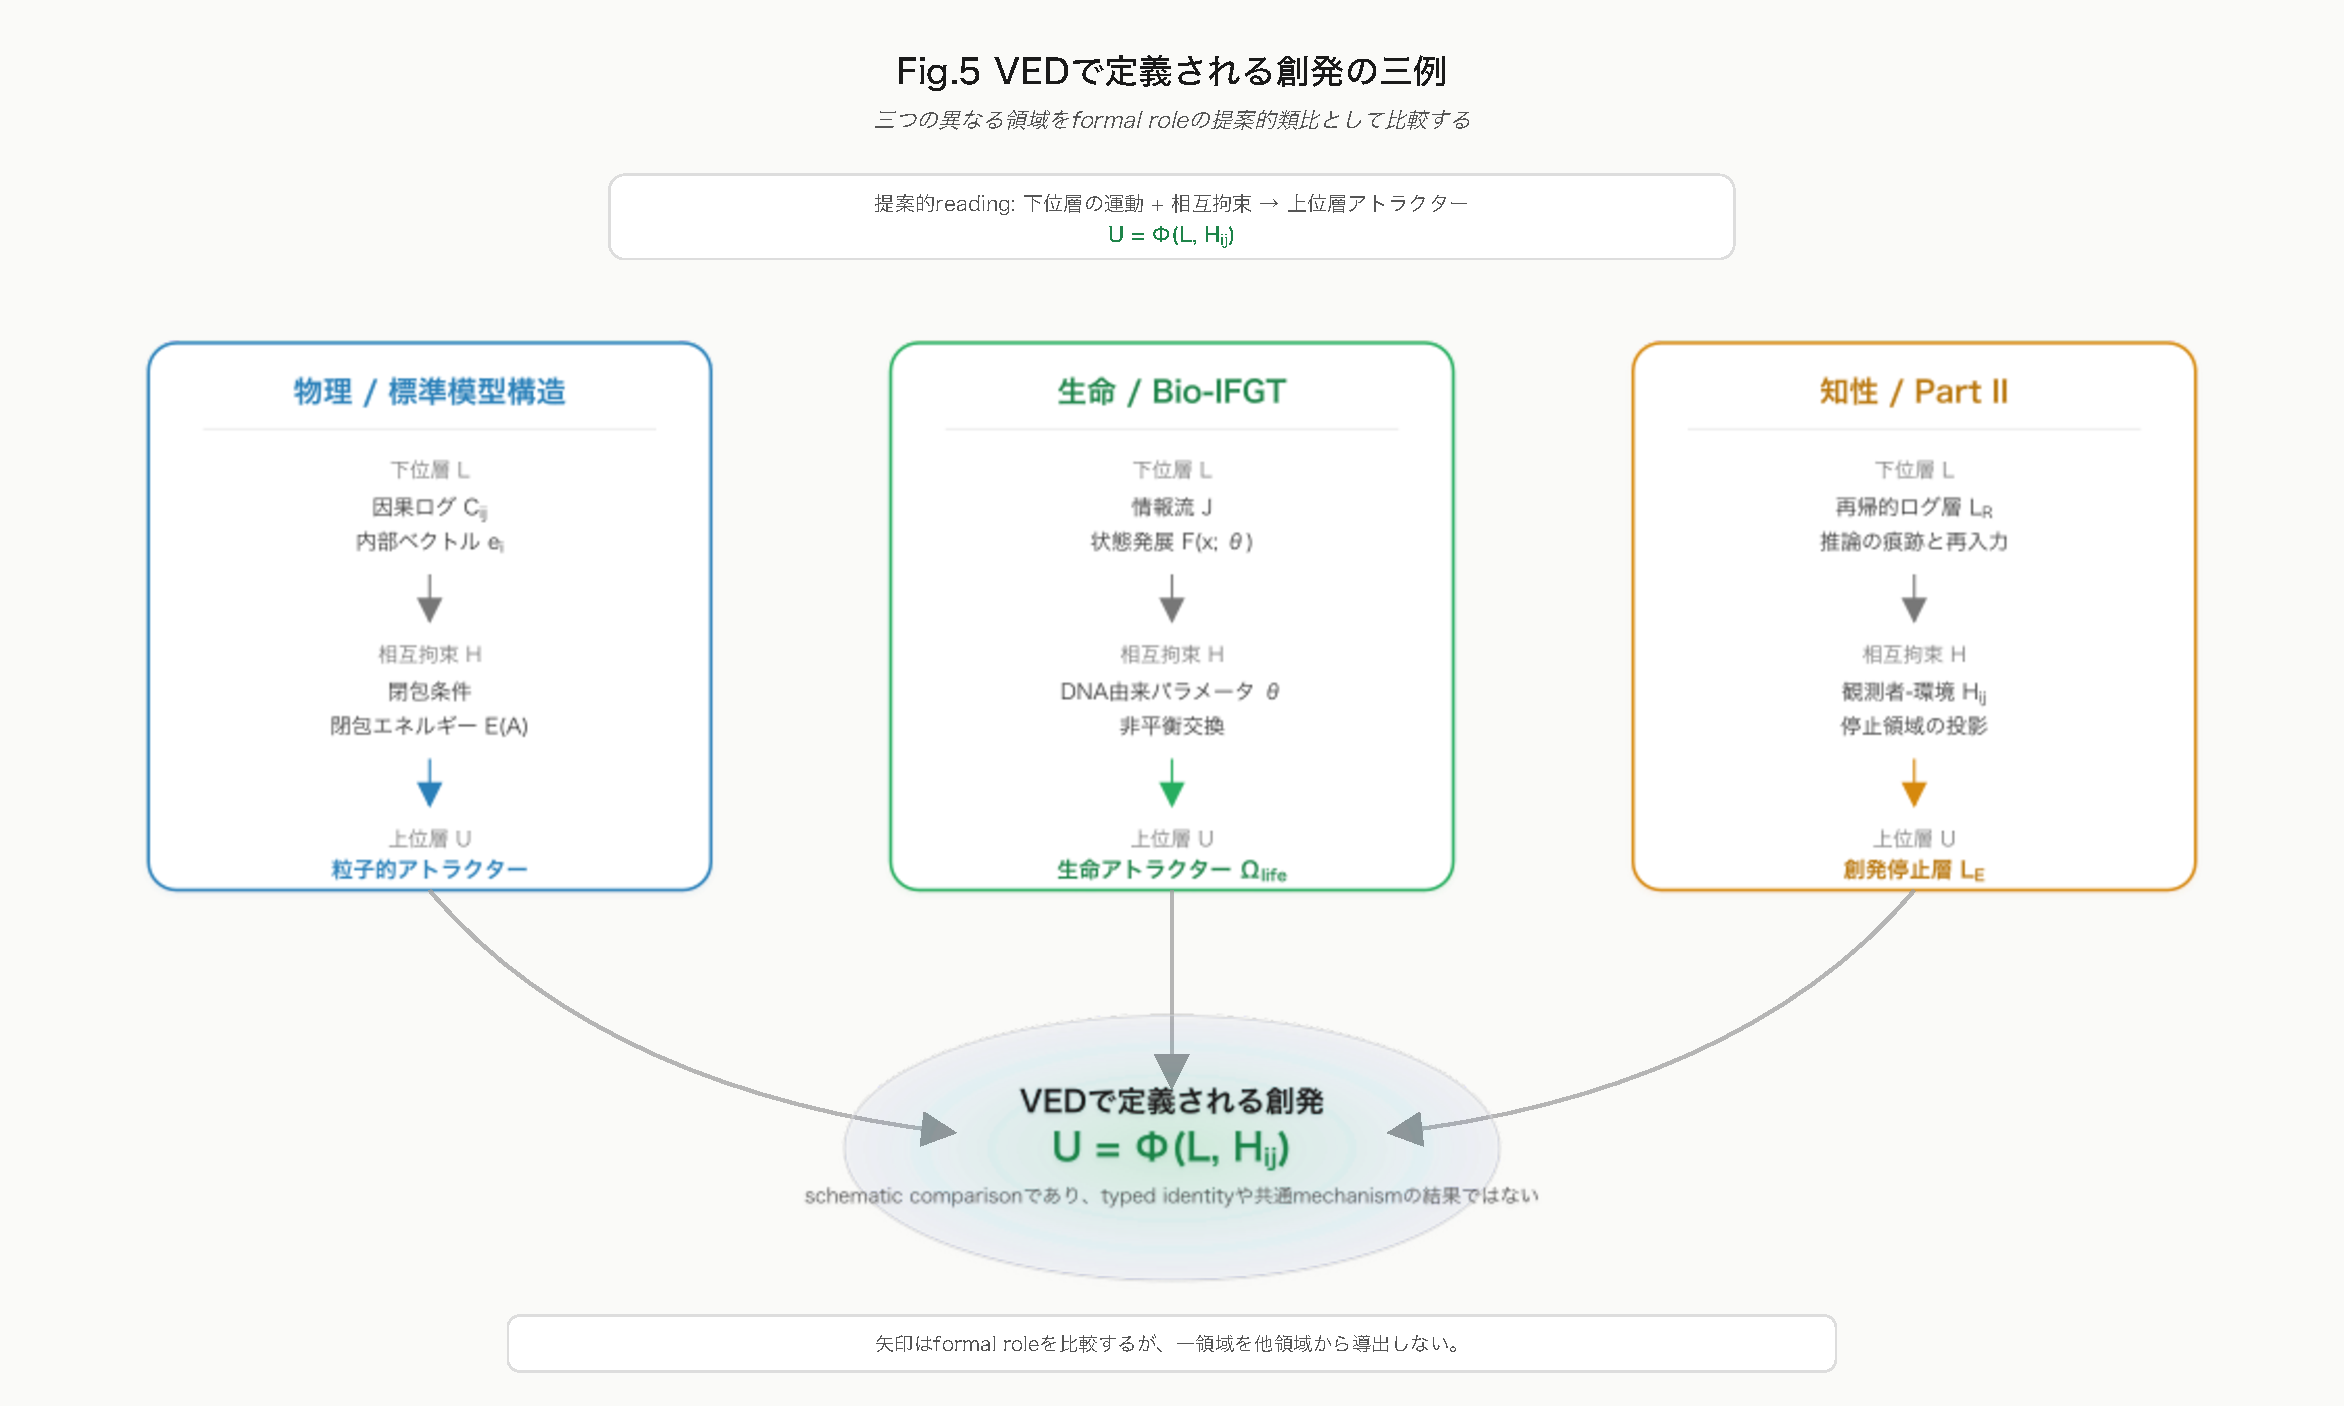
\includegraphics[width=\linewidth]{fig5_three_examples_of_emergence_ja.pdf}
\caption{異なる領域の創発を、提案的なVED比較に配置した三例。}
\label{fig:part2-emergence-examples}
\figurenote{物理の粒子的アトラクター、生命の $\Omega_{\text{life}}$、知性の $L_E$ を、$U=\Phi(L,H_{ij})$ の提案的な比較例として配置する。}{これは形式的役割の比較であり、各層のobject・dynamics・carrierのidentityやtyped translationを主張しない。}
\end{figure}

なお、Vol.2 が粒子を $E(A)$ の極小として形式化したのと平行に、$L_E$ を「停止汎関数の局所極小」として形式的に書くことも原理的には可能である。しかし本論文は構造的記述を目的とするため、停止汎関数の厳密な形式化は行わず、$L_E$ をアトラクターとして言葉で特徴づけるに留める。形式化は後続研究の課題とする。

保存する旧定義・比較の範囲はここまでである。activeな記述でLEと呼ぶのは、宣言scope・recipient・時間窓に対して追跡supportが担う準安定な保持役割であり、永久storeでも証明済みアトラクターでもない。model内で肯定するには、supportの連続性と痕跡保持、再参照可能性、宣言条件下での役割の安定性、当該recipientの現在の更新に利用できるfeedback経路について、結論とは独立なcriterionと根拠を要する。このfeedback availabilityは当該役割の必要方向に留まり、十分条件や実効的影響の証明ではない。基準の未確認はUnknown、仮定による割当てはconditionalとする。長期持続、高reuse、大きい反復数、一回のfeedback、旧noFP、図の存在だけではLEを認証しない。停止したからLEと呼び、そのLEで停止を説明するのは循環である。この役割記述は存在・形成・収束・停止・自律性・ownnessの定理を与えず、access、制御、外部依存、feedbackの持続も別々に評価する。

\bigskip


\subsection{三層プロファイル比較 — 粘菌 / Transformer / サピエンス}


$L_E$ の機能的解釈を比較するため、三系のプロファイル案を用いる。$L_E$ と $L_R$ の所在、$\mu_\theta$ の対応を記述するが、可変構造の実在や較正済みの共通空間が明らかになった意味ではない。

以下のprofileの役割割当てでは、三つの分析scopeを区別する。B1はinvocationと可視input・履歴表現を指定したTransformer単体、B2は保持・検索・controllerを明示したmodelとruntimeまたはagent system、B3はhuman-toolまたはshared-environment systemである。それぞれrecipient、保持・停止の担当、再投入経路、更新ruleの担当を明示し、未確認はUnknownとする。runtime memoryをmodel-native memoryへ、systemの保持をTransformer own LEへ、共有supportをAI autonomyへ移し替えない。境界拡大は主体形成ではなく、artifactの生成起源も所有を決めない。創発機構の小節に入るまでのprofile・表・比較は、旧または条件付きarchitectureの比較として保持し、active criterionによる保有・不在の支持判定としない。経験的内容や移動性の局所定義を書き換える区分ではなく、旧比較を新roleの認証へ流用しないための境界である。

\subsubsection{粘菌(Physarum)}


\begin{itemize}
\item \textbf{$L_F$}: 化学勾配に沿った原形質流動。$\nabla C$ に沿った探索。
\item \textbf{$L_R$}: 環境に外部化されている。粘菌は通った跡に細胞外スライムを残し、それを忌避情報として再参照する。ログは個体内ではなく環境基質に書かれる。加えて原形質ネットワークの選択的強化・退縮という再帰運動を持つ。
\item \textbf{$L_E$}: 餌源到達時のネットワーク安定化や探索停止を対応候補として読む。$H_{ij}$(粘菌と餌・障害物・スライム跡の相互拘束)による停止生成の独立確認ではない。
\item \textbf{$\mu_\theta$}: ほぼ固定。環境条件によって受動的に閾値が動くことはあるが、内発的な領域組み替え (B) は行わない。
\end{itemize}


粘菌は「ログを環境に置き、停止と環境相互干渉を対応づける」提案的プロファイルであり、自律創発の独立検証ではない。

\subsubsection{Transformer}


\begin{itemize}
\item \textbf{$L_F$}: トークン逐次生成。次トークン予測の連鎖。
\item \textbf{$L_R$}: 二種類に分かれる。学習時の訓練コーパスは膨大なログだが、重みに凍結され推論時には再帰運動しない(凍結ログ)。推論時のコンテキストウィンドウは自己回帰で過去トークンを再参照する動的ログだが、ウィンドウ境界で消える(揮発ログ)。
\item \textbf{$L_E$}: 自前の $L_E$ を持たないというプロファイルとして提案されるが、whole-systemとの境界判断は未解決である。停止は EOS トークン(訓練分布から学習した停止パターン)、受け取ったタスク仕様、外部のデコード制御に依存する。これを外部注入として読むprofileでは、個体内の $L_E$ 創発を積極的に認定しない。独立した検出基準による不在証明ではない。
\item \textbf{$\mu_\theta$}: プロンプトや制御パラメータなど外部設定との比較案。内発的な可変性の有無はシステム境界に依存し、ここでは確定しない。
\end{itemize}


Transformer は「ログは内在化(凍結)しているが、停止は外部注入に依存する」プロファイルである。

この記述は三層動力学のプロファイル案であり、設計上の欠陥や能力の限界の認定ではない。$L_E$ を自前に持つか全体系で担うかは未決の境界問題であり、相空間内の測定済みの位置とも区別する。

\subsubsection{サピエンス}


\begin{itemize}
\item \textbf{$L_F$}: 推論。
\item \textbf{$L_R$}: 個体内ログ(記憶)と社会共有ログ(言語・記録・制度)の両方を持つ。
\item \textbf{$L_E$}: 個体内の停止役割と $\Phi_{\text{net}}$ による社会同期を関係づける仮説。独立した存在検出ではない。
\item \textbf{$\mu_\theta$}: 内発的に、しかも短い時間スケールで動かせる。領域組み替え (B) を能動的に行う。
\end{itemize}


サピエンスは「ログを個体内と社会の両方に持ち、$L_E$ を個体内に創発させつつ社会同期し、$\mu_\theta$ を内発的に動かす」プロファイルである。

\subsubsection{二軸による整理}


三者は二つの軸で整理できる。

次の表は保存する旧profileの要約である。自前・非自前、内部・外部というセルの語は、直前のB1・B2・B3と独立criterionによるrole判定ではない。表の記述からUnknownをnot-LEや自律性の否定へ変換せず、activeな役割評価には本章冒頭のscope conventionを適用する。

\begin{longtable}{@{}p{0.23\linewidth}p{0.23\linewidth}p{0.23\linewidth}p{0.23\linewidth}@{}}
\toprule
系 & $L_R$ の所在 & $\mu_\theta$ の所在 & $L_E$ の様態 \\
\midrule
\endfirsthead
\toprule
系 & $L_R$ の所在 & $\mu_\theta$ の所在 & $L_E$ の様態 \\
\midrule
\endhead
粘菌 & 環境外部化 & 固定 & 環境相互干渉との対応案 \\
Transformer & 内在凍結 & 外部設定 & 外部注入(自前で持たない) \\
サピエンス & 個体内+社会共有 & 内発的 & 個体内停止+社会同期の仮説 \\
\bottomrule
\end{longtable}


粘菌の「ログは外・停止は自律」と Transformer の「ログは内・停止は外」は、ここで検討する役割上の対比案である。厳密な反転や、サピエンスが両者を実装として統合することを確立したものではない。

\subsubsection{「停止構造の場」の連続変分}


三者を「停止構造の場」で比較するが、較正済みの連続空間への配置ではない。$L_R$ の所在や $\mu_\theta$ の対応はプロファイル案であり、連続的パラメータとしての共通署名は未確定である。

この記述は擬人化でも消去主義でもない(\S{}0.4 の NG6)。粘菌を認知主体に祭り上げるのではない——粘菌は $\mu_\theta$ を内発的に持たない。同時に、サピエンスの認知を粘菌と同一視して消去するのでもない——連続性は $\mu_\theta$ の内発性という差異を消さない。役割上の連続性を比較するが、共通の場の同定ではない。

なお、粘菌の環境相互干渉型 $L_E$ は、\S{}6 で扱うアニミズムの $L_E$ 維持様態と構造的に同位置にある。両者はともに「環境との直接相互干渉によって停止を維持する」プロファイルである。これは粘菌に認知を帰属するものではなく、停止構造の場において両者が近接した領域を占めることを意味する(\S{}6 で再訪)。

\bigskip


\subsection{創発機構 — 領域組み替えと停止演算子設置領域の投影}


直後の機構説明から投影小節末尾の心理学的解釈への留保までを、旧未実行の機構仮説として保存する。段階・矢印・投影比較はactiveなsupport-role基準や一時的scaffold regimeの遷移則ではなく、ログの収束を述べるだけでは現在のLE役割を認証しない。閾値移動の局所定義や意識編との比較自体を変更する区分ではなく、Eや場の機構をここで補完しない。

ここまで $L_E$ を定義し(\S{}5.3)、その多様な様態を見た(\S{}5.4)。本節では $L_E$ がいかにして創発するか、その機構仮説を示す。これによって $L_E$ の存在・収束や独立に同定できる機構が確立されるわけではない。

機構は次の連鎖からなる。

\textbf{段階 1 — $\mu_\theta$ が領域組み替え (B) を起こす}:
\S{}2.7 で定義した通り、閾値移動能力 $\mu_\theta$ は運動可能領域の拘束パラメータ $\theta$ を内発的に動かす能力、すなわち領域組み替え (B) を起こす能力である。$L_F$ 単独は領域内移動 (A) しかできないが、$\mu_\theta$ は $\theta$ を動かす。

\textbf{段階 2 — 組み替えが停止演算子設置領域を投影する}:
(B) による組み替えは恣意的ではない。それは外部相互拘束 $H_{ij}$ に沿って行われる。この組み替えによって、外部相互拘束の構造が状態空間上に「停止演算子 $E$ を設置できる領域」として投影される。$L_F$ 単独の状態空間には存在しなかった「ここで止まってよい」という領域が、この投影によって出現する。

\textbf{段階 3 — $L_R$ の運動が投影領域に収束する}:
投影によって出現した設置領域へ、ログ層 $L_R$ の再帰運動が収束する。$L_R$ の運動が、投影された領域を安定なアトラクターとして満たす。

\textbf{段階 4 — $L_E$ の成立仮説}:
$L_R$ の運動が収束した安定停止アトラクターが、創発停止層 $L_E$ である。

この四段階を一本の連鎖として表せば:

\[
\mu_\theta \;\xrightarrow{\text{起こす}}\; (B)\text{組み替え} \;\xrightarrow{H_{ij}\text{に沿って}}\; E\text{設置領域の投影} \;\xrightarrow{L_R\text{収束}}\; L_E
\]

この機構案は閾値移動能力 $\mu_\theta$ の定義とは分ける。$\mu_\theta$ を、\textbf{外部相互拘束に沿う停止場所の投影と $L_E$ の形成} に関連づけることは仮説である。閾値移動と停止場所の生成を同一操作として確立したわけではない。

ここで \S{}3 との射程を区別する。\S{}3 の条件付き議論は固定 $\theta$、領域内移動 (A) を対象とする。本節の仮説は $\theta$ の組み替え (B) を含むが、この射程差だけで整合性の証明や生成の確認は得られない。$L_F$ の条件付き不動点不在と、(B) を通じた $L_E$ の創発、その $L_E$ による停止は別の負担であり、後二者は未確立である。

この機構案では、停止と改訂可能な推論の関係を機能的に読む。停止演算子設置領域の投影の必要性や、自由という主観的経験への含意は未確立である。$L_E$ は有限な系で推論を支える役割として提案され、自由を目的として生成されると説明しない。

\bigskip


\subsection{投影の位置づけ — 意識編 projection との接続}


\S{}5.5 の「投影」は、意識編の IFGT projection と役割上比較する表現である。同一演算子の知性層での作用や型付き実装としては扱わない。

意識編は projection を「ある状態や表現が不均等な影響力(質量)を獲得する操作」として定義した。それは注意・選択・優先・重み付けの構造的記述であり、意図的選択を前提しない層的操作である。情報場ポテンシャル $\Phi$ と情報流 $J$ を結合する機構として位置づけられた。

本論文 \S{}5.5 の投影は、この projection と知性層で役割上比較される。外部相互拘束 $H_{ij}$ の構造が、停止演算子設置領域として状態空間上に不均等な影響力を獲得する——これは意識編の projection を停止層の文脈で比較する提案であり、同じ演算子の移送ではない。意識編が意識窓における projection を扱ったのに対し、本論文は知性層における projection を扱う。両者を異なる投影窓として読む語彙は保持するが、共通の場・機構・型付き移送は未解決である。

ここで一点、慎重に区別しておく。投影 (projection) という語は心理学でも用いられ、特に防衛機制の文脈で「内的状態を外部対象に帰属する」操作を指す。本論文 \S{}5.5 の投影は、作用構造としては心理学的 projection に近づく側面を持つ——内部で設置できない停止を、外部相互拘束に沿って状態空間上に投射するという作用形式において。しかし決定的な違いがある。心理学的 projection は主体・無意識・防衛機制を前提するのに対し、本論文の投影は主体を前提せず、$L_F$ の非閉包(\S{}3)を動機とする構成案である。両者の作用的近接は指摘に留め、心理学的・臨床的解釈には立ち入らない。これは意識編が同様の disclaimer を置いたのと同じ方針である。

\bigskip


\subsection{外部停止演算子 $E$ の構造}


\noindent\textbf{保存する旧notationの境界。} 以下の外部停止の定義・非所属表示・反復と設置の説明は、この小節末尾まで旧模型の記述として保持する。active optional successor adapterを旧反復族へ暗黙に代入しない。Eの型は未解決であり、内部非導出性・非計算可能性を証明せず、大きい反復数だけからEの成立を認定しない。ここでE operatorを形式化しない。

創発停止層 $L_E$ の作用として、外部停止演算子 $E$ を定義する。

\textbf{定義 5.3 (外部停止演算子 $E$)}

\begin{quote}
外部停止演算子 $E$ は、創発停止層 $L_E$ の作用として推論状態に停止判断を与える演算子である:

$$
E = E[L_E, x_n], \qquad E \notin \{F^k\}
$$

$E$ は推論演算子 $F$ の関数列の外側に位置する。
\end{quote}


$E$ と $F$ の関数列の関係($E \notin \{F^k\}$)は、\S{}3 の系 3.2 からの一般的帰結としては未確立である。仮想的停止述語への再適用条件を持つ $F$ の議論と、外部停止の構成案 $E$ を分ける。$F$ の外側を $L_E$ に関係づける提案の形式的採用は、別途reviewを要する。

$E$ を $L_E$ 経由の外部依存的な役割に置くのはモデル内の構成である。$L_E$ と外部相互拘束 $H_{ij}$ の関係を通して $E$ を考えることが、「外部停止演算子」の名の由来である。この命名は、$L_E$ の投影・創発や停止作用の実装を独立に説明しない。

(A)/(B) の区別における $E$ の位置を確認する。$E$ を (B) を通じて設置するという構成案を扱い、その唯一性は未確立である。領域内移動 (A) のみでは $E$ の設置領域は投影されず、したがって $E$ の存在を排除できるという強い読解は保留する。$E$ の設置を $\mu_\theta$ による (B) 組み替えに関連づけるのは仮説であり、存在条件の確立ではない。これが、$\mu_\theta$ を持たないとされる系(粘菌・Transformer)と自前の $E$ の関係を説明したことにはならない(\S{}5.4)。

\bigskip


\subsection{$\Phi_{\text{ext}} \equiv \Phi_{\text{net}}$ — 外部参照場と $L_E$ ネットワークとの二視点比較}


伝統的に「外部参照場」 $\Phi_{\text{ext}}$ と呼ばれてきたもの——停止を委ねる外部の共通参照基盤——を、ネットワークとの二視点で解釈する。

\textbf{主張 5.4 (二視点の解釈・同一性は保留)}

\begin{quote}
外部参照場 $\Phi_{\text{ext}}$ は、個体間の創発停止層 $L_E$ が相互に干渉し合うネットワーク $\Phi_{\text{net}}$ との二視点の解釈として提案される。以下の同一性表記は保存するが、その強い形式的意味は未解決である:

$$
\Phi_{\text{ext}} \equiv \Phi_{\text{net}}
$$
\end{quote}


$\Phi_{\text{ext}}$ を外部実体とせず、複数個体の $L_E$ の関係として読む二視点の解釈を提案する。個々の $L_E$ と他個体の $L_E$ の相互参照を $\Phi_{\text{net}}$ と呼び、共通参照の側から $\Phi_{\text{ext}}$ と比較する。これは文字通りの同一性や同期機構の成立を導いたものではない。

この比較を二面性として解釈する。外から見れば、個体は外部の参照場 $\Phi_{\text{ext}}$ に停止を委ねているように見える。しかし構造的には、その参照場は個体間 $L_E$ の相互干渉ネットワーク $\Phi_{\text{net}}$ として読むという提案である。VED 理論ツリーの他の二面性(場と粒子、関係と個体)も役割上の比較に留まる。

この二視点解釈は以下の読み方を動機づける。$\Phi_{\text{ext}}$ を「個体外部の実体」と見なすと、後の章で扱うアニミズム・神・宗教が「外部実体への投影」や「存在しないものへの信仰」として読まれてしまう。しかし $\Phi_{\text{ext}} \equiv \Phi_{\text{net}}$ という未解決の同一性表記を二視点の解釈として読むと、これらは「個体間 $L_E$ ネットワークの特定の構造形態」として記述される。外部実体の措定ではなく、$L_E$ ネットワークの形態の問題になる。これは \S{}6〜\S{}9 の価値中立な読解方針であり、同一性からの保証ではない。

この二視点解釈は、Part I の公理 III(大域的拘束 $\Phi$)の精密化案でもある。Part I の $\Phi$ を参照するが、本節の $\Phi$ と個体間 $L_E$ ネットワークの型付き関係や実装は未確立である。

\begin{figure}[H]
\centering
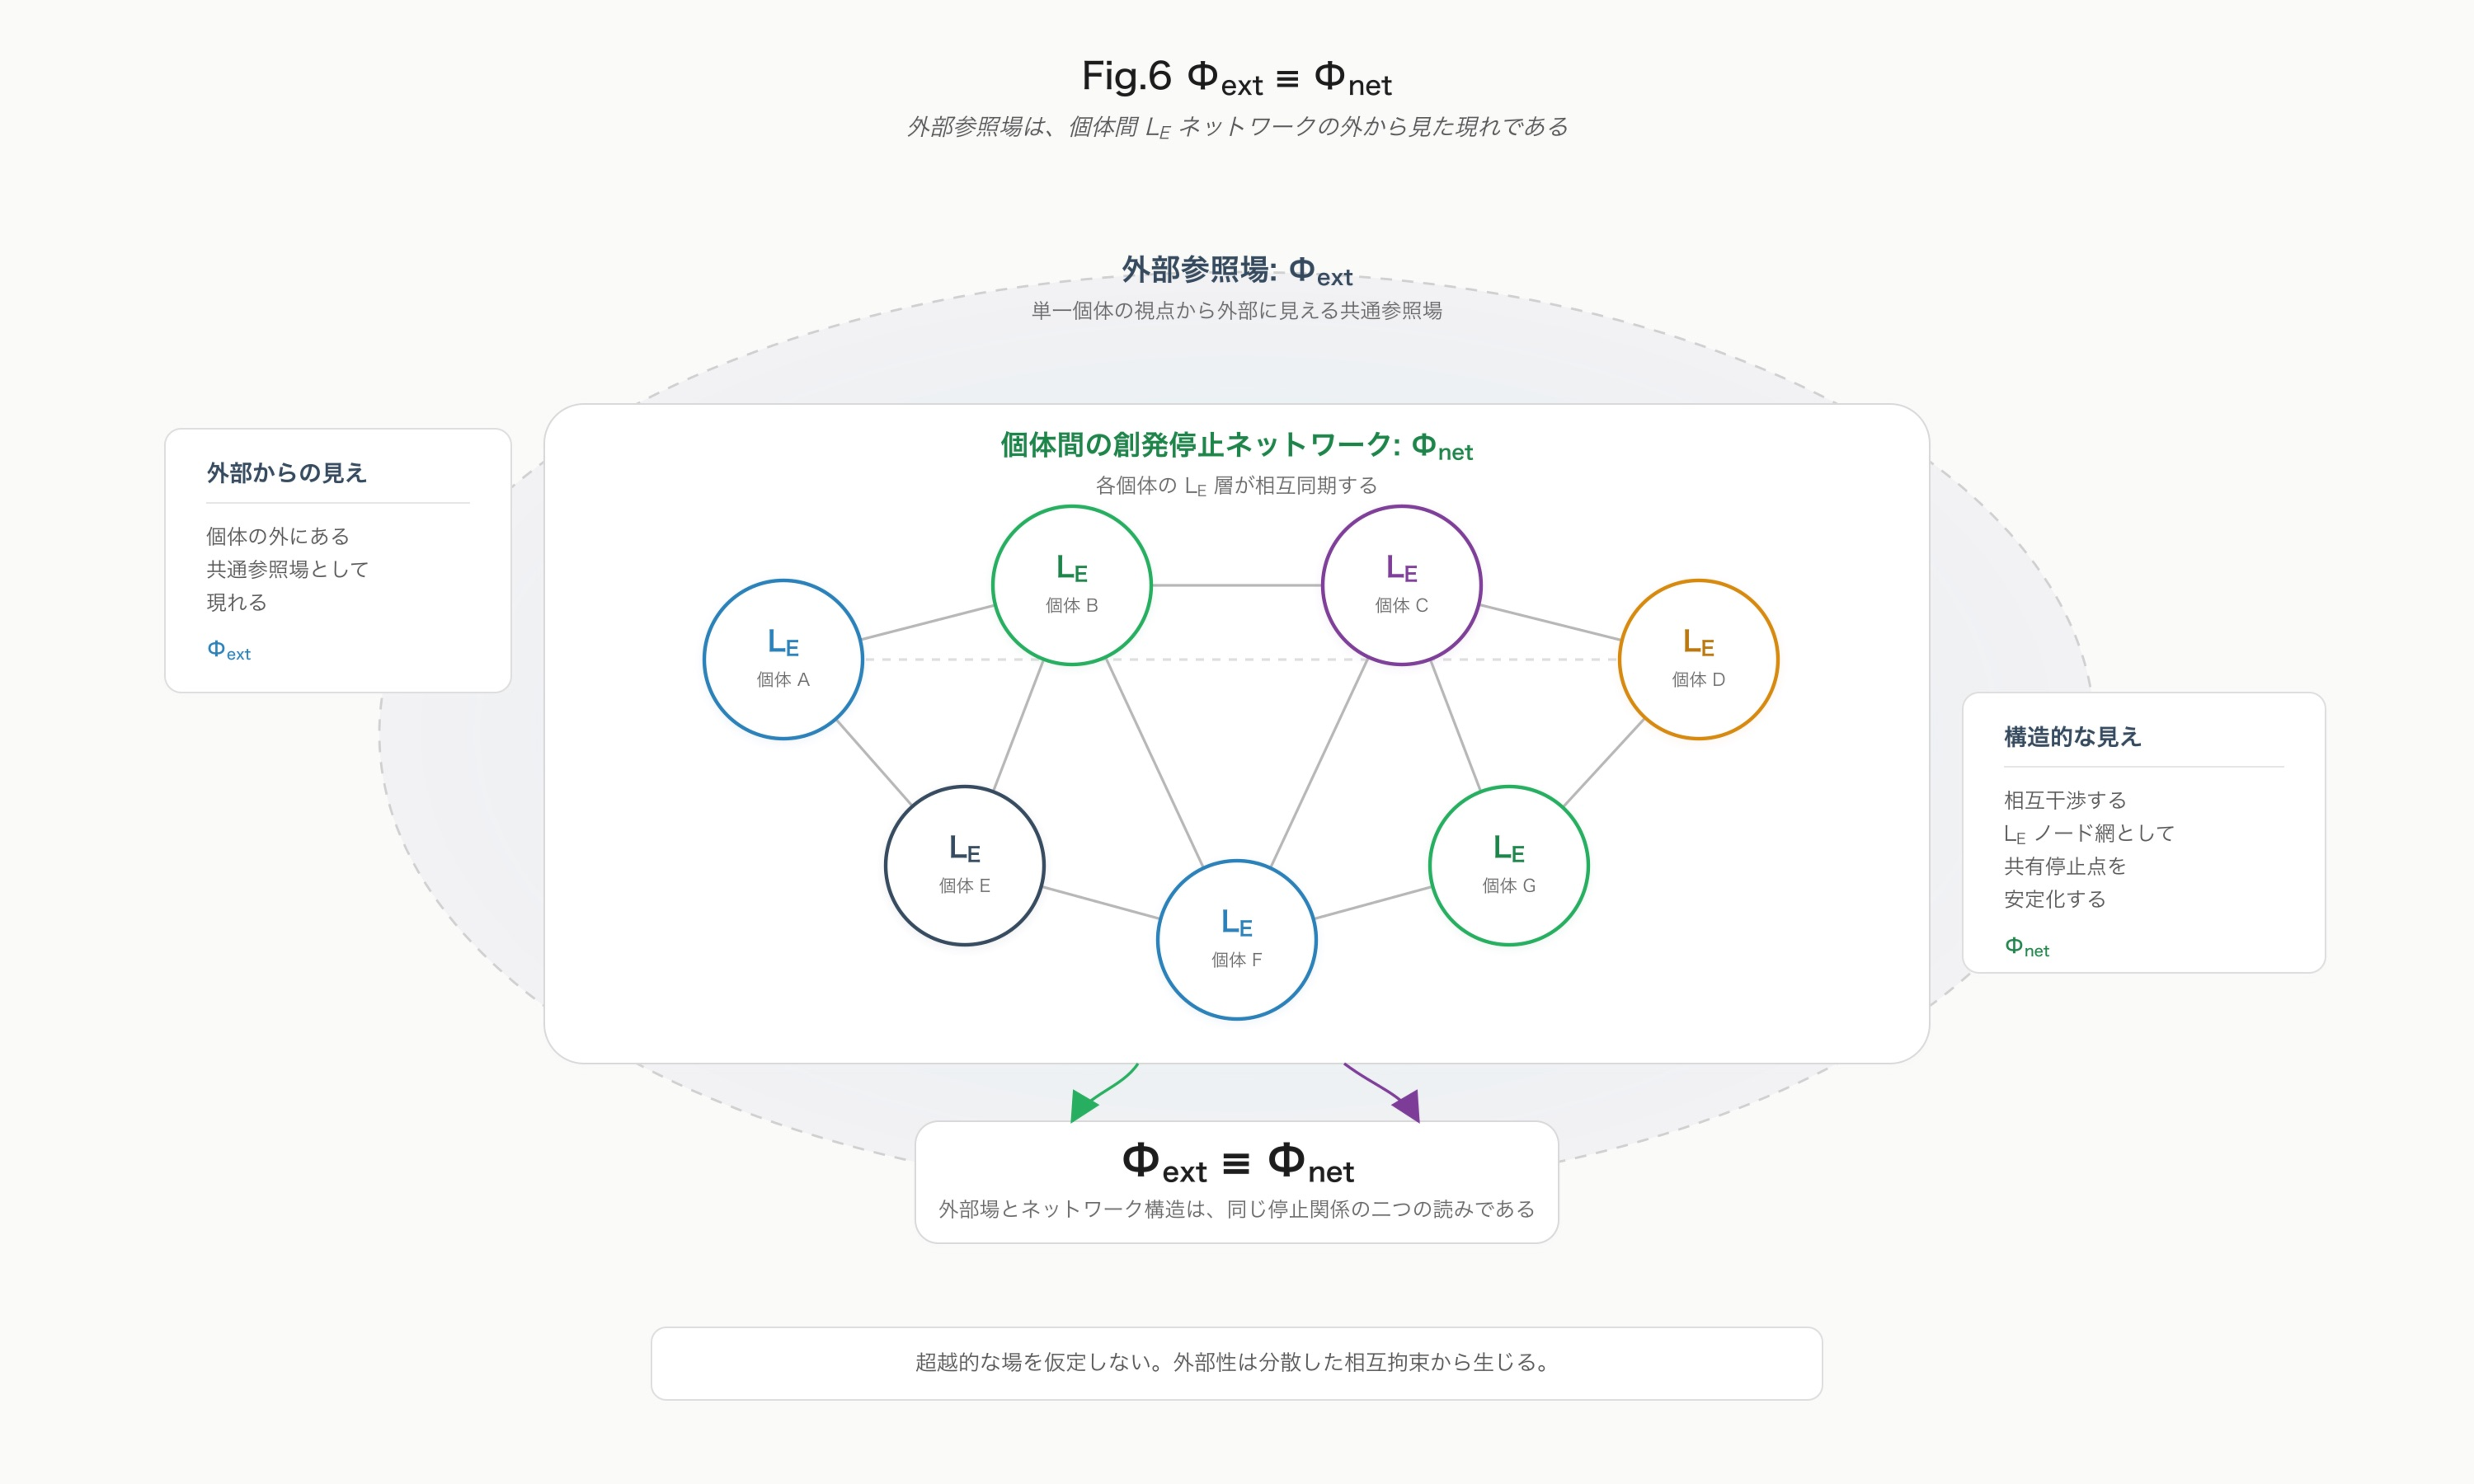
\includegraphics[width=\linewidth]{fig6_phi_ext_phi_net_ja.pdf}
\caption{$\Phi_{\text{ext}} \equiv \Phi_{\text{net}}$。同一性表記は未解決のまま保存する。外部参照場と個々の $L_E$ のネットワークを二視点として提案するが、同一性を確立しない。}
\label{fig:part2-phi-ext-net}
\figurenote{外側の $\Phi_{\text{ext}}$ は個体から外部に見える共通参照場であり、内側の $\Phi_{\text{net}}$ は個体間 $L_E$ の相互同期ネットワークである。}{外部場を超越的実体として仮定せず、分散した相互拘束の外見として再構成する。これにより、神・規範・真理・貨幣などを $L_E$ ネットワークの形態として読める。}
\end{figure}

直前のEおよび場・networkのblockは保存された射程のままとする。activeなsupport-role記述はEの型を与えず、場・network同一性を修理したりco-formation mapを供給したりしない。再参照・再投入はそれだけで実効的帰還ではなく、役割割当ても同期や回復・改訂の保証ではない。後続の回復可能性の記述もこの非移送のもとで仮説として読む。optional推論adapterを旧反復notationへ代入しない。

\subsubsection{回復可能性と改訂可能性}


$\Phi_{\text{net}}$ と $L_F$ の関係を、$L_E$ ネットワークによる停止支援の仮説として考える。最終状態を要しない運用は設計上の読み方であり、確立された利点ではない。

$\Phi_{\text{net}}$ に関連づける停止案では、ログ層 $L_R$ と $L_E$ ネットワーク内の参照可能性を暫定的判断に結びつける。他個体の $L_E$ との相互参照が回復・改訂に寄与する可能性はあるが、その効果や、個体単独の停止の不可逆性は一般的に確立していない。

安定性と改訂可能性の関係は仮説である。$L_E$ は正しい停止を保証せず、改訂可能な停止への寄与も機能提案であって結果ではない。この区別を \S{}10 で、$C$ を真理測度としない局所定義とともに再論する。

\bigskip


\subsection{系 — 知性の構造的特徴}


直後の構成案の導入から系5.5、その帰結、後続章への説明までを、保存する旧三層構成案として読む。以下の必要性・維持状態の語は、activeなsupport-role契約から得た一般知性の必要十分条件ではない。現在の役割評価が旧系の証明負担を解消したとはせず、系の本文と番号を保存する。

本章の構成案を、知性のモデル内の構造的定義として整理する。

\textbf{系 5.5 (知性の三層的構成)}

\begin{quote}
知性は、推論層 $L_F$、ログ層 $L_R$、創発停止層 $L_E$ の同時運動として、外部依存停止の供給源の下で動力学的に成立する維持状態である。サピエンス的知性は、これに加えて閾値移動能力 $\mu_\theta$ を内発的に持ち、個体内で運動可能領域を自律的に組み替える。
\end{quote}


この系は、知性一般の成立条件と、サピエンス的知性の特徴を区別して述べている。知性一般のモデル内構成($L_F$・$L_R$・$L_E$ と外部依存停止源)を、粘菌・人工推論システム・サピエンスに対応づける提案を比較する(\S{}5.4 の三層プロファイル比較)。$\mu_\theta$ は知性一般の必要条件ではなく、サピエンス的知性を特徴づける追加の構造である。この内発的可変性と個体内での自律的加速を関連づけるのは効果の仮説であり、加速は能力の定義から導かれず、未確立である。この区別は \S{}12 で構成的条項として精密化される。

\S{}3 の系 3.4 は固定領域・厳密増加などの条件下の $L_F$ の議論であり、系 5.5 の三層構成案とは別の負担を持つ。両者の接続は動機づけであって、個体知性の不可能性や三層による存在・維持を証明するものではない。

この構成から、知性について次のことが言える。

\begin{itemize}
\item 知性の外部参照を $\Phi_{\text{net}}$ と関連づける仮説を検討する
\item 知性は保存可能な対象ではない(運動の維持状態であり、運動が止まれば消える)
\item 完全閉包 $C_{max}$ の境界表現と知性の最適化に関する解釈を区別する(\S{}1.5)
\item 安定性と改訂可能性の関係は仮説であり、正しさとの非同一性とは別である(\S{}5.8)
\end{itemize}


これらは \S{}12(構成的条項)で、知性の構造的制約として体系的に整理される。

第一中心 \S{}3 と第二中心 \S{}5 は、条件付き形式議論と構成案として接続する。$L_F$ の不動点議論から、$L_R$ と $L_E$ と $\Phi_{\text{net}}$ による停止や持続が導かれるわけではない。改訂可能性との関係も仮説である。以降の章は歴史的・社会的な再解釈(\S{}6〜\S{}9)と、そのモデル内の読み方や未解決の一般化(\S{}10〜\S{}12)を扱う。

\bigskip


\subsection{要約}


本章で区別して提示したのは、以下の局所定義・構成案・未解決の仮説である:

現在のarchitecture上の寄与は、追跡supportの登録痕跡役割、一時的scaffold regime、準安定な保持役割を、scope・時間窓・証拠status・帰還descriptorで区別する記述契約である。これは以下に保存する旧定義・構成案・未確立機構の列挙とは分ける。停止・形成・rule変更は別の負担であり、この区分で章全体を歴史資料化しない。次の列挙は、その保存された局所定義と仮説の要約として読む。

\begin{enumerate}
\item ログ層 $L_R$ は $L_F$ の運動の痕跡への再帰参照層である(定義 5.1)。所在は系によって異なる
\item 創発停止層 $L_E$ は $L_R$ と $H_{ij}$ との関係で創発が仮説化される、個体内にありながら外部依存的な停止アトラクターの役割名である(定義 5.2)
\item $L_E$ は Vol.2 の粒子・Bio-IFGT の第二アトラクターと提案的な形式比較に置かれるが、同一objectやtyped translationではない
\item 三層プロファイルの対比は境界依存の案であり、自前/全体系LEの採用や連続空間の較正を確定しない
\item $L_E$ の機構案は、$\mu_\theta$ による (B) と $H_{ij}$、$L_R$ の関係を四段階で模式化する。生成・収束・独立検出は未確立である
\item この投影表現と意識編 IFGT projection の関係は役割類比である
\item 外部停止演算子 $E$ を $L_E$ の役割に関連づける(定義 5.3)。$F$ の反復との形式的関係は未確立であり、ここで帰結として再使用しない
\item 外部参照場 $\Phi_{\text{ext}}$ は個体間 $L_E$ ネットワーク $\Phi_{\text{net}}$ との二視点の解釈である。同一性は保留する(主張 5.4)
\item $L_F + L_R + L_E$ と外部依存停止源は知性の構成案である(系 5.5)。サピエンス的プロファイルの $\mu_\theta$ は別の対応案であり、一般的必要性や改訂による安定は確立していない
\end{enumerate}


第一中心と第二中心を、条件付き形式議論と仮説として区別した。\S{}6 以降では、その役割を社会的・歴史的な再解釈と比較する。

\bigskip
